\documentclass{beamer}
\usetheme[pageofpages=of,% String used between the current page and the
                         % total page count.
          bullet=circle,% Use circles instead of squares for bullets.
          titleline=true,% Show a line below the frame title.
          alternativetitlepage=true,% Use the fancy title page.
          titlepagelogo=logo-circl.pdf,% Logo for the first page.
%          watermark=watermark-polito,% Watermark used in every page.
%          watermarkheight=100px,% Height of the watermark.
%          watermarkheightmult=4,% The watermark image is 4 times bigger
                                % than watermarkheight.
          ]{Torino}

\usepackage[utf8]{inputenc}
\usepackage{xcolor}
\usepackage{tikz}
\usepackage{listings}
\usepackage{array}
\usepackage{colortbl}
\usetikzlibrary{positioning}
\usetikzlibrary{shapes,arrows,snakes,automata,positioning,matrix,fit}
%\usetikzlibrary{shapes,arrows}
\usepackage{appendixnumberbeamer}
%\usepackage[T1]{fontenc}
%\usepackage[scaled]{beramono}

\author{\small{Team CIRCL\\G{\'e}rard Wagener \\ \emph{TLP:CLEAR}}}
\title{Analysis Techniques of Executable and Linkable Format (ELF)}
\subtitle{MISP-LEA project}

\institute{\href{https://www.circl.lu}{https://www.circl.lu} \\}
\date{20 January, 2025}
\begin{document}

\begin{frame}
    \maketitle
\end{frame}
\begin{frame}{What is ELF?}
    \begin{itemize}
        \item ELF stands for Executable and Linkable Format\footnote{\url{https://refspecs.linuxfoundation.org/elf/elf.pdf}}.
        \item It is a common standard file format for executables, object code, shared libraries, and core dumps.
        \item Originally developed by Unix System Laboratories and now widely used in Unix-like operating systems.
    \end{itemize}
\end{frame}

\begin{frame}{Structure of an ELF File}
    \begin{itemize}
        \item An ELF file consists of three main parts:
        \begin{itemize}
            \item \textbf{Header:} Contains metadata about the file type, architecture, and entry point.
            \item \textbf{Program Header Table:} Describes how the file should be loaded into memory.
            \item \textbf{Section Header Table:} Provides information about the sections in the file.
        \end{itemize}
        \item ELF files are designed to be flexible and extensible.
    \end{itemize}
\end{frame}

\begin{frame}{Benefits of ELF}
    \begin{itemize}
        \item Platform-independent format, enabling portability.
        \item Simplifies the linking and loading process.
        \item Supports dynamic linking, reducing redundancy.
        \item Extensively used in modern development environments.
    \end{itemize}
\end{frame}

\begin{frame}[fragile]
\frametitle{Binwalk Output}

\begin{lstlisting}[language=bash, basicstyle=\ttfamily, breaklines=true]
Sample: 6420f5d7d48b75d687b8356e93c82721bb536c633d773f8985f74c8977425f04

binwalk sample
\end{lstlisting}

\begin{tabular}{ccp{0.6\textwidth}}
\textbf{Decimal} & \textbf{Hexadecimal} & \textbf{Description}\\
0                & 0x0                  & ELF, 32-bit LSB executable, Intel 80386, version 1 (SYSV) \\
13111            & 0x3337               & Boot section Start 0x58028941 End 0x5A41 \\
13115            & 0x333B               & Boot section Start 0x5A41 End 0x0 \\
\end{tabular}

\vspace{1cm}

$\to$ matched signatures
\end{frame}

\begin{frame}[fragile]
\frametitle{Using Binwalk}
\framesubtitle{Sample: 9e70725640c4284e2049e4b25c9cc46cca496053cebf69855ec25acc9bd63e05}
\begin{tabular}{|c|c|p{0.6\textwidth}|}
\hline
\textbf{Decimal} & \textbf{Hexadecimal} & \textbf{Description} \\ \hline
0                & 0x0                  & ELF, 64-bit LSB executable, AMD x86-64, version 1 (GNU/Linux) \\ \hline
600864           & 0x92B20              & Unix path: /usr/share/locale \\ \hline
612774           & 0x959A6              & Unix path: /usr/lib/getconf \\ \hline
620336           & 0x97730              & Unix path: /usr/lib/locale \\ \hline
622368           & 0x97F20              & Unix path: /usr/lib/locale/locale-archive \\ \hline
674903           & 0xA4C57              & Unix path: /usr/lib/x86\_64-linux-gnu/ \\ \hline

\textbf{778039}           & \textbf{0xBDF37}              & \textbf{mcrypt 2.2 encrypted data, algorithm: blowfish-448, mode: CBC, keymode: 8bit} \\ \hline
\end{tabular}

\end{frame}

\begin{frame}
\frametitle{Using Binwalk}

\begin{itemize}
    \item \textbf{Encrypted Data:}
    \begin{itemize}
        \item The file contains data encrypted using \textbf{mcrypt 2.2}.
    \end{itemize}
    \item \textbf{Encryption Algorithm:}
    \begin{itemize}
        \item Algorithm: \textbf{Blowfish-448}, a symmetric block cipher with a 448-bit key size.
    \end{itemize}
    \item \textbf{Cipher Mode:}
    \begin{itemize}
        \item Mode: \textbf{CBC (Cipher Block Chaining)} for enhanced security via block interdependency.
    \end{itemize}
    \item \textbf{Key Mode:}
    \begin{itemize}
        \item Key processed in \textbf{8-bit mode}, possibly a default for mcrypt configurations.
    \end{itemize}
    \item \textbf{Implications:}
    \begin{itemize}
        \item Decryption requires the encryption key and potentially an initialization vector (IV).
        \item Indicates sensitive or protected data within the file.
        \item Poses a reverse engineering challenge without the key.
    \end{itemize}
\end{itemize}

\end{frame}

\begin{frame}[fragile]
\frametitle{Extracting the content}
Sample: 9e70725640c4284e2049e4b25c9cc46cca496053cebf69855ec25acc9bd63e05
\begin{lstlisting}[language=bash, basicstyle=\ttfamily, frame=single, breaklines=true]
dd if=sample of=extracted_data bs=1 skip=778039
\end{lstlisting}

\begin{itemize}
    \item Binwalk uses signatures to identify and extract data from files.
    \item Determine the size of the detected block for further analysis.
    \item Evaluate whether the detection is a false positive by inspecting the data manually or using additional tools.
\end{itemize}

\end{frame}


\begin{frame}[fragile]
\frametitle{ELF Symbols from Binary Analysis}

Extract symbols from binary excluding GBLIBC references

Sample: 6420f5d7d48b75d687b8356e93c82721bb536c633d773f8985f74c8977425f04
\begin{lstlisting}[language=bash, basicstyle=\ttfamily, frame=single]
nm sample | grep -v GBLIBC
\end{lstlisting}


\begin{lstlisting}[basicstyle=\ttfamily, frame=single]
08048bfd t p4tch_sel1nux_codztegfaddczda
08048e9c t parse_cred
8050bb3 T prepare_fops_lsm_shellcode
08049215 t put_your_hands_up_hooker
0804b220 D r1ngrrrrrrr
0804988e t rey0y0code
0804b2c0 d ruujhdbgatrfe345
\end{lstlisting}
\end{frame}

\begin{frame}
\frametitle{ELF Symbols from Binary Analysis}

\begin{itemize}
    \item Interpretation of the output of tool \tt{nm}
    \item man page is your friend
\end{itemize}

\begin{tabular}{|c|p{0.7\textwidth}|}
\hline
\textbf{Symbol Type} & \textbf{Explanation} \\ \hline
a & The symbol's value is absolute and will not be changed by further linking. \\ \hline
b & The symbol is in the BSS data section. \\ \hline
d & The symbol is in the initialized data section. \\ \hline
r & The symbol is in the read-only data section. \\ \hline
t & The symbol is in the text (code) section. \\ \hline
w & The symbol is a weak symbol that has not been specifically tagged as a weak object symbol. \\ \hline
\end{tabular}

\end{frame}

\begin{frame}[fragile]
\frametitle{Using objdump to View ELF Sections}

\begin{lstlisting}[language=bash, basicstyle=\ttfamily, frame=single, breaklines=true]
objdump -h sample
\end{lstlisting}

\begin{itemize}
    \item \textbf{Output Structure:}
    \begin{itemize}
        \item Lists all sections in the ELF file, including their attributes.
        \item Provides information such as:
        \begin{itemize}
            \item \textbf{Idx}: Section index in the ELF file.
            \item \textbf{Name}: Name of the section (e.g., `.text`, `.data`).
            \item \textbf{Size}: Size of the section in bytes.
            \item \textbf{VMA (Virtual Memory Address)}: Where the section is loaded in memory.
            \item \textbf{File Off}: Offset of the section in the binary file.
            \item \textbf{Attributes}: Flags indicating section properties (e.g., `ALLOC`, `LOAD`, `READONLY`).
        \end{itemize}
    \end{itemize}
    \item \textbf{Use Case:}
    \begin{itemize}
        \item Identify key sections like `.text` (code), `.data` (initialized data), `.bss` (uninitialized data), and `.dtor` (destructors).
        \item Useful to identify the type of binary, such as a C program, C++, Go (Golang), etc. 
    \end{itemize}
\end{itemize}

\end{frame}



\begin{frame}[fragile]
\frametitle{ELF Section Details}

\begin{tabular}{clcccp{1cm}}
\textbf{Idx} & \textbf{Name}       & \textbf{Size}  & \textbf{VMA}     & \textbf{LMA}     & \textbf{File Off} \\
0            & .interp            & 00000013       & 08048134         & 08048134         & 00000134          \\
1            & .note.ABI-tag      & 00000020       & 08048148         & 08048148         & 00000148          \\
2            & .gnu.hash          & 00000030       & 08048168         & 08048168         & 00000168          \\
3            & .dynsym            & 00000290       & 08048198         & 08048198         & 00000198          \\
11           & .text              & 00001788       & 080489b0         & 080489b0         & 000009b0          \\

\end{tabular}

\vspace{1cm}

\begin{tabular}{cc}
\textbf{Idx} &  \textbf{Attributes}\\
0            &  CONTENTS, ALLOC, LOAD, READONLY, DATA \\
1            &  CONTENTS, ALLOC, LOAD, READONLY, DATA \\
2            &  CONTENTS, ALLOC, LOAD, READONLY, DATA \\
3            &  CONTENTS, ALLOC, LOAD, READONLY, DATA \\
11           &  CONTENTS, ALLOC, LOAD, READONLY, \textbf{CODE}
\end{tabular}

\end{frame}

\begin{frame}
\frametitle{Collaborative Malware Analysis Using MISP}

\centering
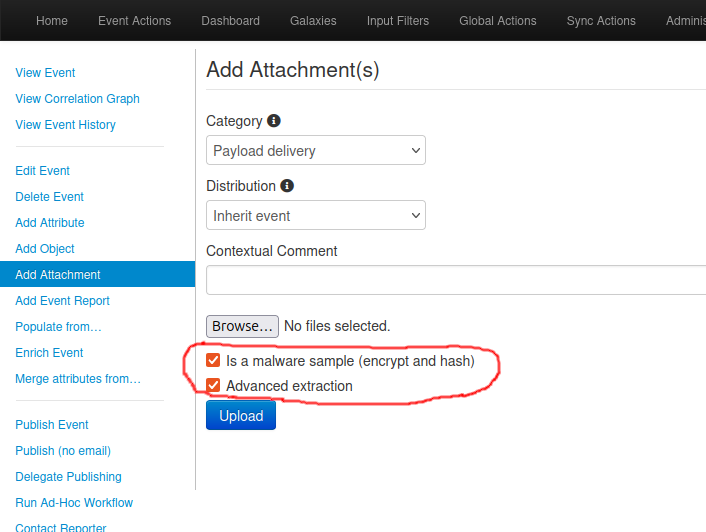
\includegraphics[width=0.8\textwidth]{img/upload2.png}

Uploading your sample to MISP

\end{frame}

\begin{frame}
\frametitle{Collaborative Malware Analysis Using MISP}

\centering
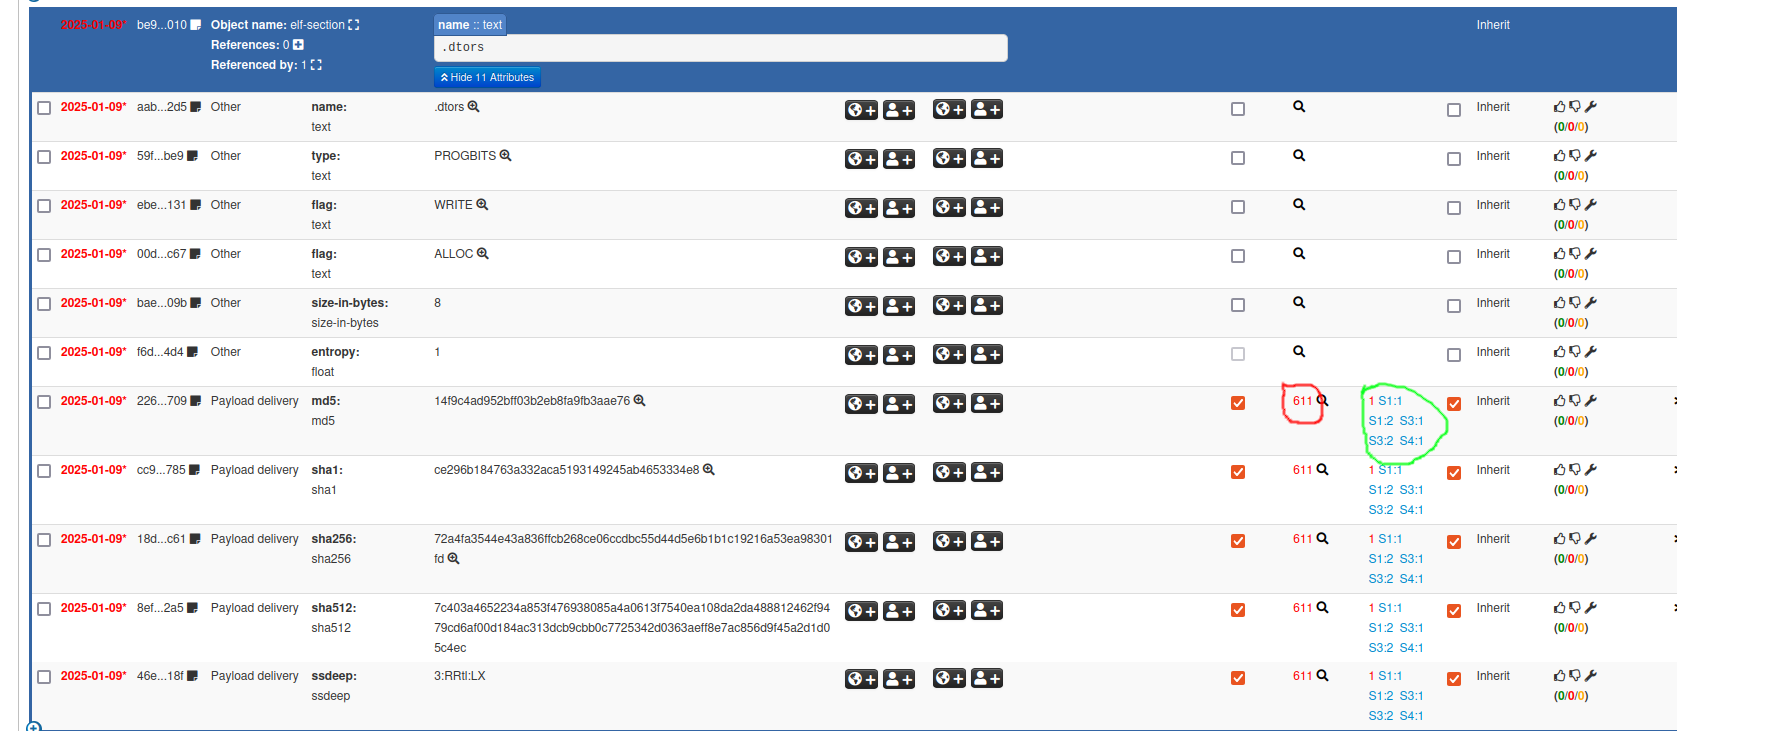
\includegraphics[width=0.8\textwidth]{img/correlation2.png}

\begin{itemize}
    \item Explore correlations between events and indicators.
    \item Analyze results from threat intelligence feeds.
    \item Review hits from synchronization caches.
    \item Watch out for false positives. Check the size of the section, as smaller sizes are more susceptible to false positives.
\end{itemize}

\end{frame}

\begin{frame}
\frametitle{Collaborative Malware Analysis Using MISP}

Exploring connected MISP instances within MISP-LEA

\centering
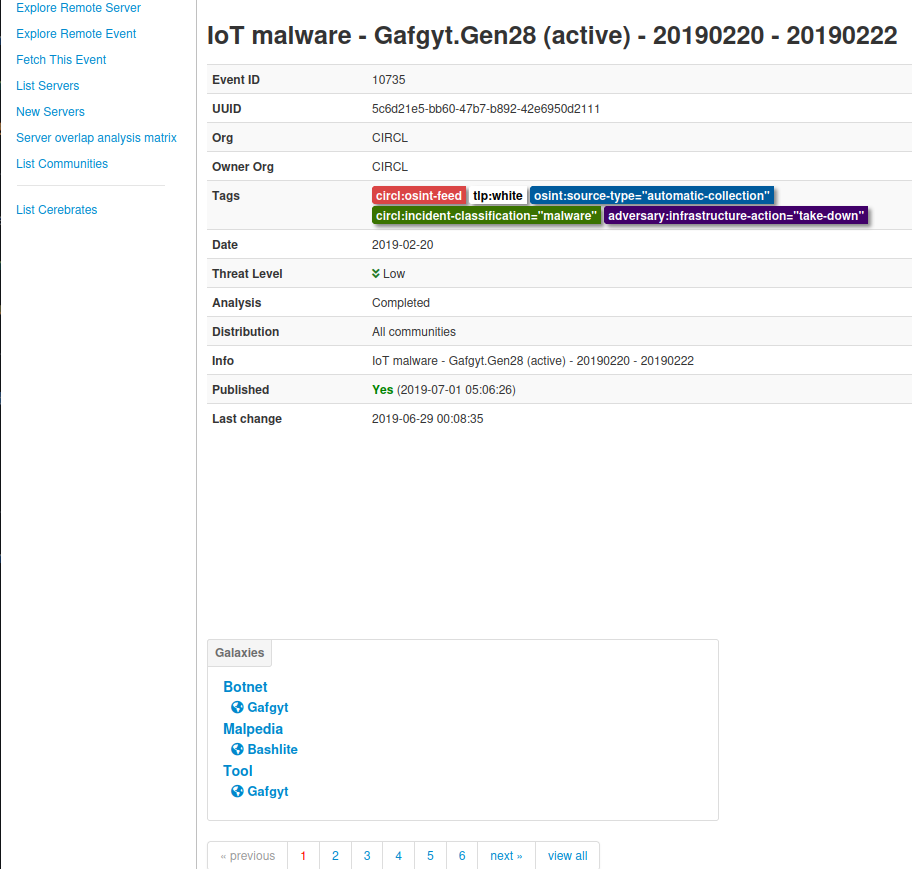
\includegraphics[width=0.6\textwidth]{img/foreign.png}

\end{frame}


\begin{frame}[fragile]
\frametitle{Disassembly of $<$main$>$ (Part 1) with objdump}
\begin{verbatim}
8049d05 <main>:
8049d05: 8d 4c 24 04            lea   0x4(%esp),%ecx
8049d09: 83 e4 f0               and   $0xfffffff0,%esp
8049d0c: ff 71 fc               push  -0x4(%ecx)
8049d0f: 55                     push  %ebp
8049d10: 89 e5                  mov   %esp,%ebp
8049d12: 51                     push  %ecx
8049d13: 83 ec 34               sub   $0x34,%esp
8049d16: 89 4d e4               mov   %ecx,-0x1c(%ebp)
8049d19: c7 04 24 cc a5 04 08   movl  $0x804a5cc,(%esp)
8049d20: e8 37 ec ff ff         call  804895c <puts@plt>
8049d25: e8 82 eb ff ff         call  80488ac <getuid@plt>
8049d2a: 85 c0                  test  %eax,%eax
\end{verbatim}
\end{frame}

\begin{frame}[fragile]
\frametitle{Disassembly of $<$main$>$ (Part 2) with objdump}

\begin{verbatim}
8049d47: c7 04 24 42 a6 04 08   movl  $0x804a642,(%esp)
8049d4e: e8 89 eb ff ff         call  80488dc <fwrite@plt>
8049d53: c7 45 e8 01 00 00 00   movl  $0x1,-0x18(%ebp)
8049d5a: e9 1c 03 00 00         jmp   804a07b <main+0x376>
8049d5f: 8b 55 e4               mov   -0x1c(%ebp),%edx
8049d62: 8b 42 04               mov   0x4(%edx),%eax
8049d65: 89 44 24 04            mov   %eax,0x4(%esp)
8049d69: 8b 55 e4               mov   -0x1c(%ebp),%edx
8049d6c: 8b 02                  mov   (%edx),%eax
8049d6e: 89 04 24               mov   %eax,(%esp)
8049d71: e8 e2 f8 ff ff         call  8049658 <env_prepare>
8049d76: e8 59 fa ff ff         call  80497d4 <y0y0stack>
8049d7b: e8 b1 fa ff ff         call  8049831 <y0y0code>
\end{verbatim}

\end{frame}




\begin{frame}
\frametitle{Introduction Ghidra}

\begin{itemize}
    \item \textbf{Disassembly and Decompilation:}
    \begin{itemize}
        \item Transforms binary code into human-readable assembly.
        \item Generates high-level language representations (C-like pseudocode).
    \end{itemize}
    \item \textbf{Cross-Platform Support:}
    \begin{itemize}
        \item Analyzes binaries for multiple architectures (x86, ARM, MIPS, etc.).
        \item Compatible with various operating systems (Windows, Linux, macOS).
    \end{itemize}
    \item \textbf{Collaboration:}
    \begin{itemize}
        \item Supports multi-user reverse engineering projects.
        \item Version-controlled changes for shared analysis.
    \end{itemize}
    \item \textbf{Scriptability:}
    \begin{itemize}
        \item Customize and automate analysis with Python and Java.
    \end{itemize}
    \item \textbf{Extensibility:}
    \begin{itemize}
        \item Add plugins and extend functionality for specific needs.
    \end{itemize}
    \item \textbf{Data Flow Analysis:}
    \begin{itemize}
        \item Tracks variables, functions, and references for better insight.
    \end{itemize}
\end{itemize}

\end{frame}

\begin{frame}
\frametitle{Static Analysis Using Ghidra}
\begin{itemize}
    \item Creating a project in Ghidra.
    \item Importing and analyzing a binary file.
\end{itemize}

\centering
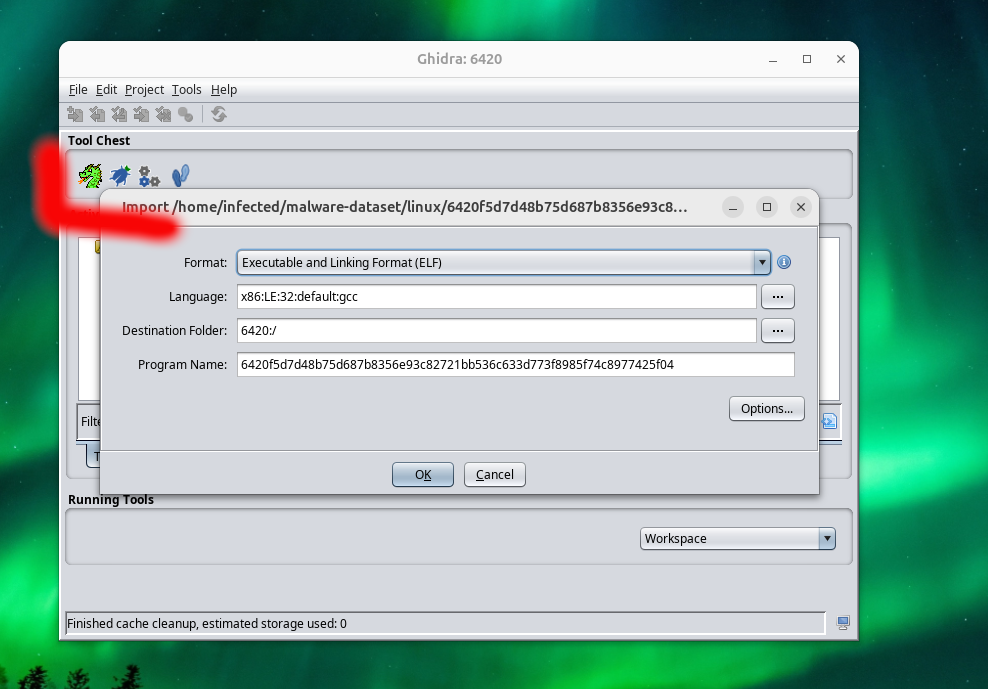
\includegraphics[width=0.6\textwidth]{img/g0.png}

\end{frame}

\begin{frame}
\frametitle{Static Analysis Using Ghidra}

\begin{itemize}
    \item Determine the type of binary (e.g., ELF, PE).
    \item Analyze the binary's metadata for key attributes such as architecture, endianness, and sections.
\end{itemize}

\centering
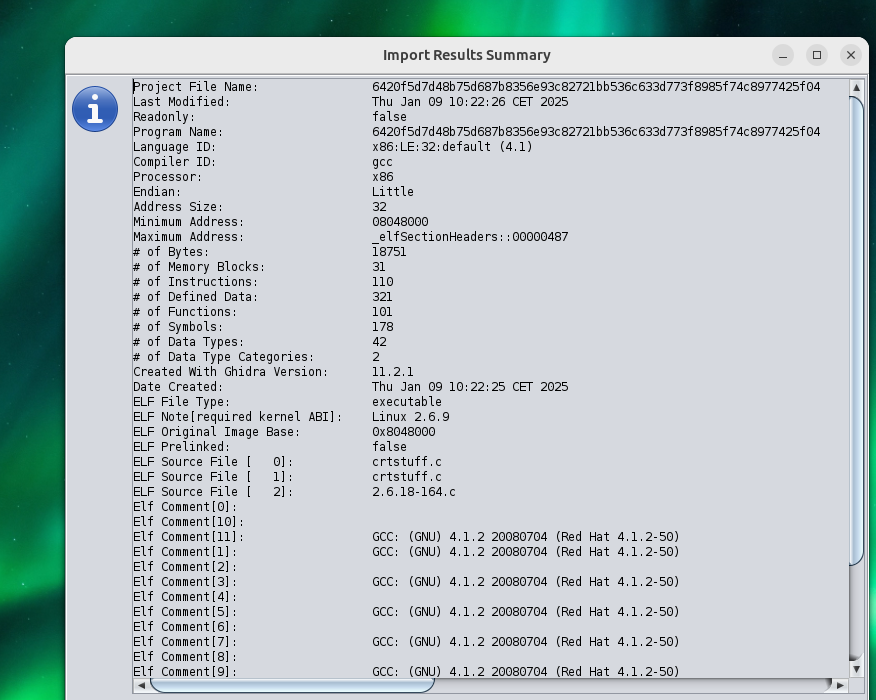
\includegraphics[width=0.6\textwidth]{img/g1.png}
\end{frame}

\begin{frame}
\frametitle{Static Analysis Using Ghidra}

\begin{itemize}
    \item Explore the functions defined within the binary.
    \item Analyze the disassembly view to examine low-level instructions.
    \item Utilize the decompiled view for a high-level representation of the code.
\end{itemize}

\centering
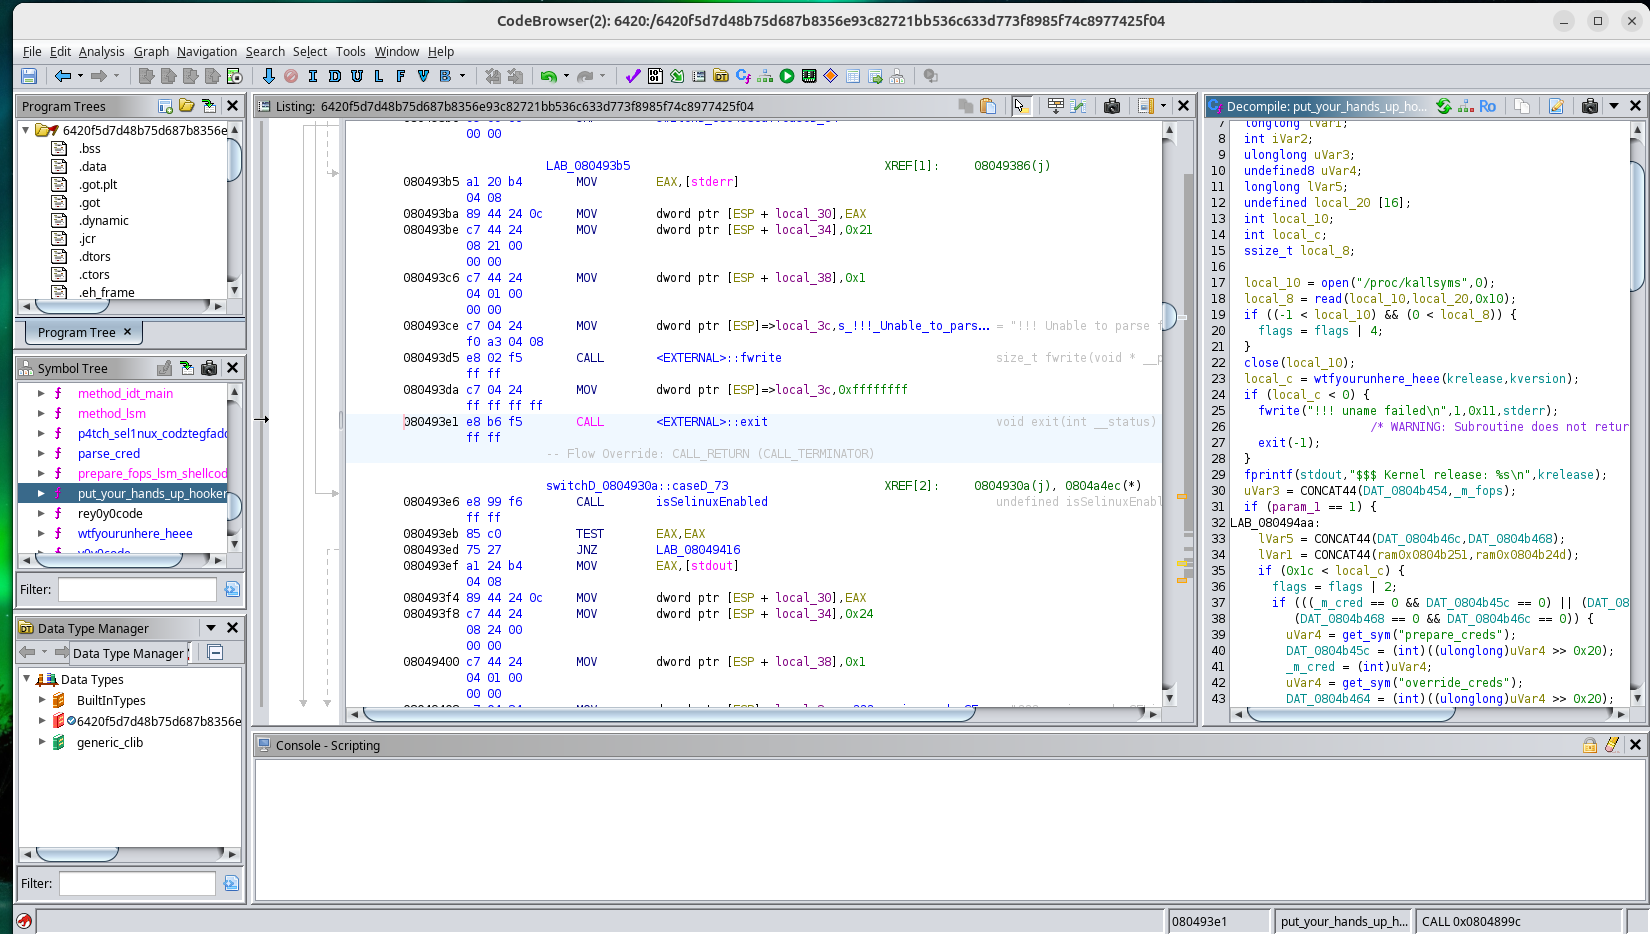
\includegraphics[width=0.6\textwidth]{img/g2.png}
\end{frame}

\begin{frame}
\frametitle{Static Analysis Using Ghidra}

\begin{itemize}
    \item \textbf{Benefits of Ghidra's Decompiled View:}
    \begin{itemize}
        \item Provides a high-level, human-readable representation of the code.
        \item Simplifies understanding of complex binaries.
    \end{itemize}
    \item \textbf{Avoid Manual Pattern Matching:}
    \begin{itemize}
        \item Eliminates the need to manually match patterns in assembly code.
        \item Speeds up the reverse engineering process.
    \end{itemize}
\end{itemize}

\centering
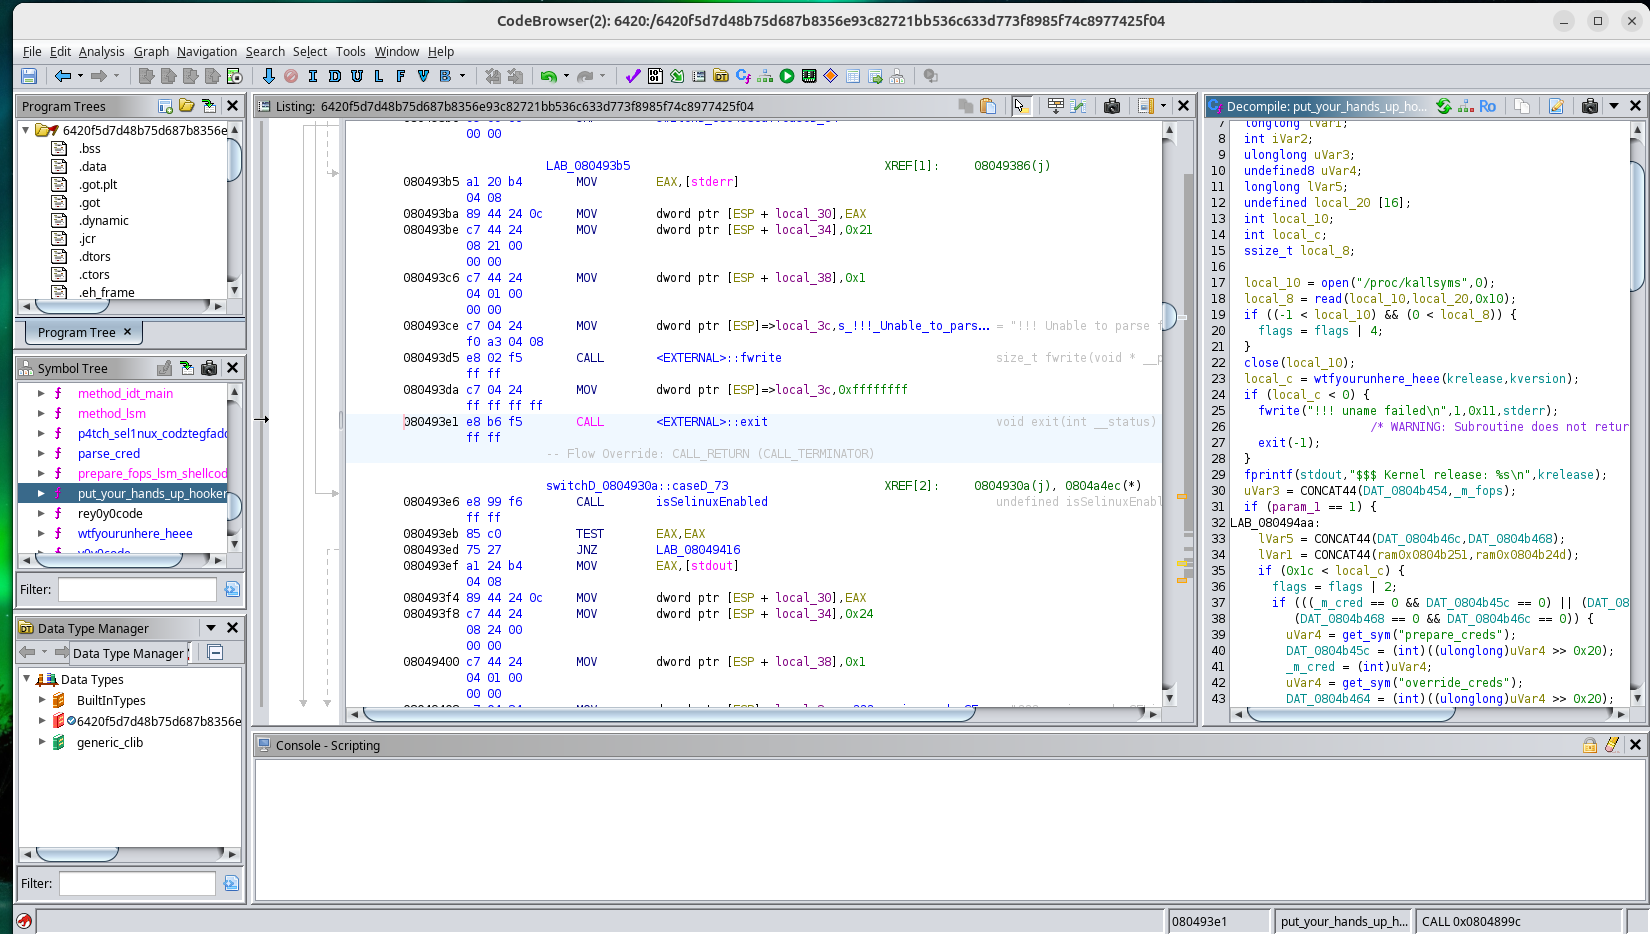
\includegraphics[width=0.6\textwidth]{img/g2.png}
\end{frame}

\begin{frame}
\frametitle{String Analysis and Cross-References in Ghidra}

\begin{itemize}
    \item Identify interesting strings, such as filenames, hardcoded paths, or error messages.
    \item Use the cross-references (Xrefs) feature to determine which functions or code sections utilize these strings.
\end{itemize}

\centering
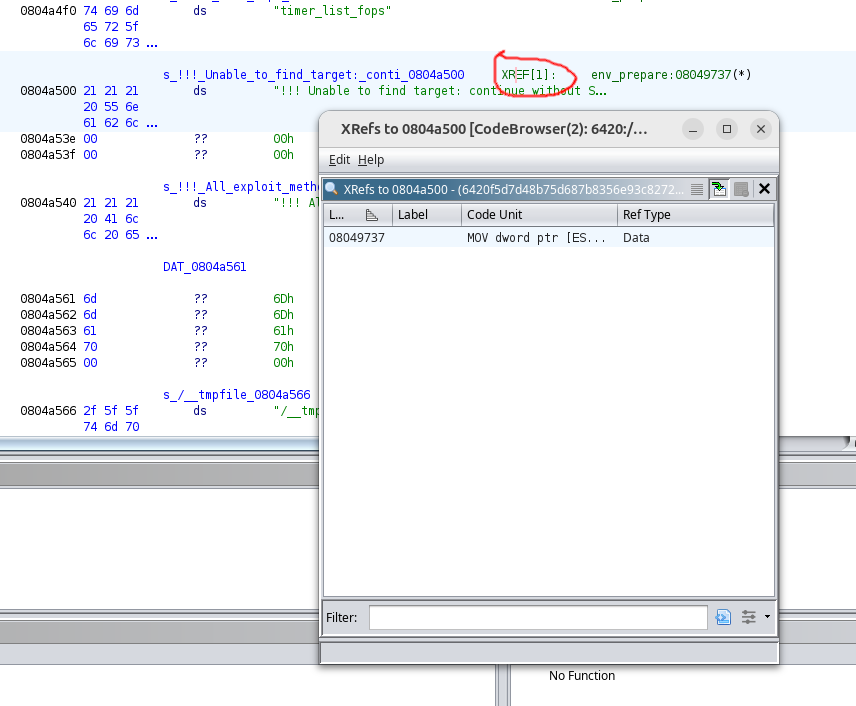
\includegraphics[width=0.6\textwidth]{img/gxref.png}
\end{frame}


\begin{frame}
\frametitle{String Analysis and Function Call Trees in Ghidra}

\begin{itemize}
    \item Certain functions are known to generate forensic artifacts, such as `fopen` and `mmap`.
    \item Locate these functions in the function call tree to identify which functions use them.
    \item Determine the artifacts that can be leveraged for detection and analysis.
\end{itemize}

\centering
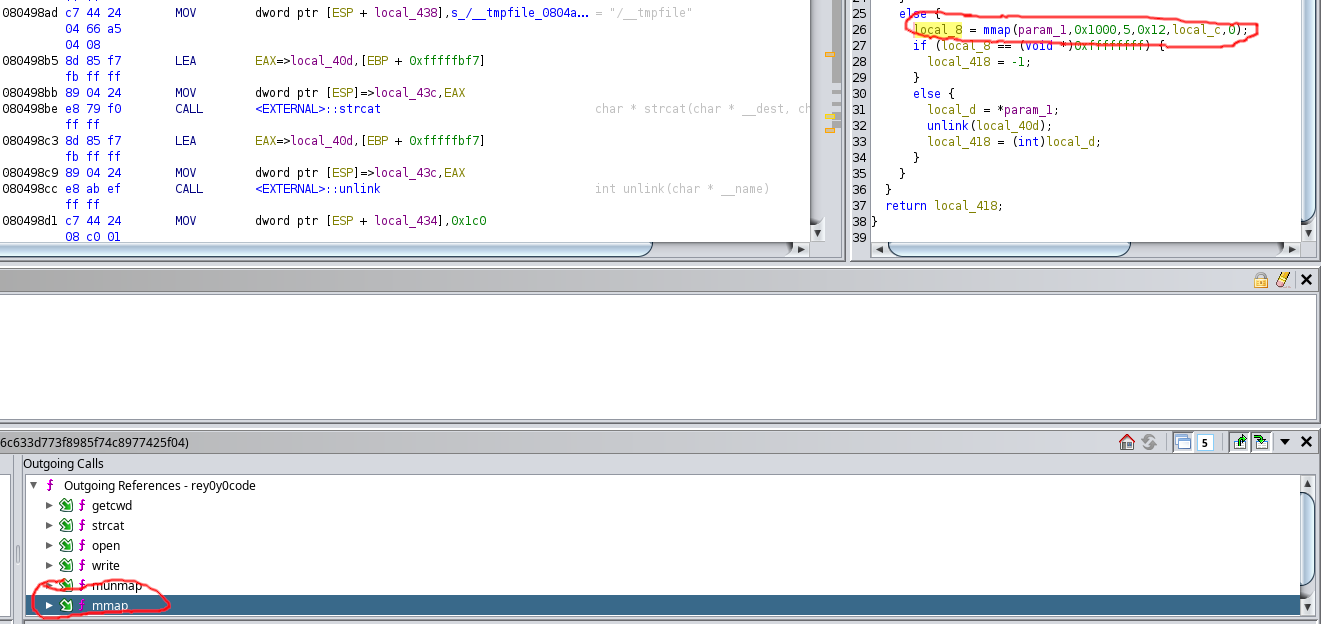
\includegraphics[width=0.6\textwidth]{img/goutcall.png}
\end{frame}


\begin{frame}
\frametitle{Static Analysis and Function Call Graphs in Ghidra}

\begin{itemize}
    \item Visual representations of function call graphs provide valuable insights into program behavior.
    \item Insights include identifying parsing activities, code execution loops, and function relationships.
\end{itemize}

\centering
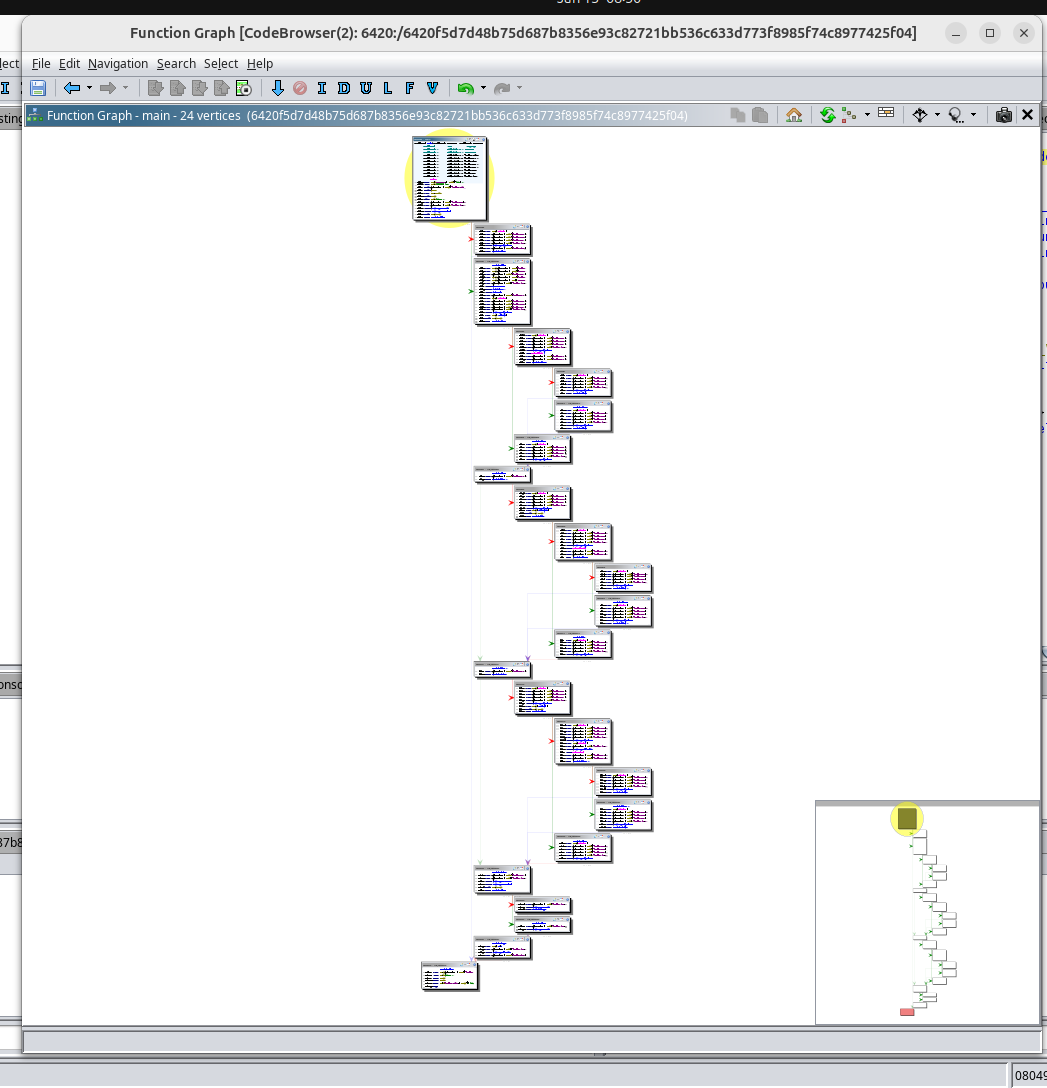
\includegraphics[width=0.6\textwidth]{img/gfctg.png}
\end{frame}

\begin{frame}
\frametitle{Core Dumps on Ubuntu}

\begin{itemize}
    \item \textbf{What is a Core Dump?}
    \begin{itemize}
        \item A core dump is a snapshot of a program's memory at the moment it crashes.
        \item Used for debugging to analyze the cause of the crash.
    \end{itemize}

    \item \textbf{Where to Find Core Dumps in Ubuntu?}
    \begin{itemize}
        \item Default location: \texttt{/var/lib/apport/coredump}.
        \item When using \texttt{systemd}, they may be in \texttt{/var/lib/systemd/coredump}.
        \item Core dumps may also be written to the program's working directory or as specified by \texttt{/proc/sys/kernel/core\_pattern}.
    \end{itemize}

    \item \textbf{Configuring Core Dumps:}
    \begin{itemize}
        \item Set unlimited size: \texttt{ulimit -c unlimited}.
        \item Check core pattern: \texttt{cat /proc/sys/kernel/core\_pattern}.
        \item Enable or configure core dumps in \texttt{/etc/security/limits.conf}.
    \end{itemize}
\end{itemize}

\end{frame}

\begin{frame}[fragile]
\frametitle{Analyzing Crash Reports}

\textbf{Problem Type:} Crash \\
\textbf{Architecture:} amd64 \\
\textbf{Crash Counter:} 1 \\
\textbf{Date:} Thu Jan 9 15:51:49 2025 \\

\textbf{Dependencies:}
\begin{itemize}
    \item adduser 3.137ubuntu1
    \item adwaita-icon-theme 46.0-1
    \item apt 2.7.14build2
    \item apt-utils 2.7.14build2
    \item at-spi2-common 2.52.0-1build1
    \item at-spi2-core 2.52.0-1build1
    \item base-passwd 3.6.3build1
    \item ca-certificates 20240203
    \item dbus 1.14.10-4ubuntu4.1
    \item dbus-bin 1.14.10-4ubuntu4.1
    \item dbus-daemon 1.14.10-4ubuntu4.1
    \item dbus-session-bus-common 1.14.10-4ubuntu4.1
    \item dbus-system-bus-common 1.14.10-4ubuntu4.1
    \item dconf-cli 0.40.0-4build2
\end{itemize}

\end{frame}

\begin{frame}[fragile]
\frametitle{Analyzing a Base64-Encoded Core Dump}

\textbf{Crash Report Details:}
\begin{itemize}
    \item \textbf{Source Package:} zoom
    \item \textbf{System Info:} Linux 6.8.0-51-generic x86\_64
    \item \textbf{User Groups:} adm, cdrom, dip, kvm, libvirt, lpadmin, plugdev, sudo, users
    \item \textbf{Core Dump Format:} Base64 Encoded
\end{itemize}

\textbf{Base64 Blob (Partial):}
\begin{verbatim}
H4sICAAAAAAC/0NvcmVEdW1wAA==
7J0HgBPV2v5nYUGaGhuiog5WLECogqJEEQVBjCiKlSy7C6y0sLsgYIsFxZ5r78Te
74169drQ2LnW2LvGjj2Wq
\end{verbatim}

\textbf{Note:} Decode the Base64 blob to retrieve the original core dump using the following command:
\begin{verbatim}
echo "H4sICAAAAAAC/0NvcmVEdW1wAA==" | base64 -d > coredump.gz
gunzip coredump.gz
\end{verbatim}

\end{frame}

\begin{frame}
\frametitle{Extracting Core Dumps from Crash Files}

\begin{itemize}
    \item Unzipping the core dump creates a file such as \texttt{\_opt\_zoom\_ZoomWebviewHost.1000.crash}.
    \item Decoding and decompressing the binary blob will produce a core dump.
\end{itemize}


\begin{block}{Extracted Core Dump Details}
\textbf{Format:} ELF 64-bit LSB core file, x86-64 \\
\textbf{Details:} SVR4-style, from \texttt{/opt/zoom/ZoomWebviewHost --type=utility --utility-sub-type=screen\_ai.mojom.Scr} \\
\textbf{User Info:} real uid: 1000, effective uid: 1000, real gid: 1000, effective gid: 1000 \\
\textbf{Exec Path:} \texttt{/opt/zoom/ZoomWebviewHost} \\
\textbf{Platform:} x86\_64
\end{block}

\textbf{Note:} Use tools like \texttt{gdb}, \texttt{readelf}, or \texttt{objdump} to analyze the extracted core dump.

\end{frame}

\begin{frame}[fragile]
\frametitle{Setting up Kaitai Struct}

\begin{itemize}
    \item The latest release (as of 2022) is available on GitHub:
          \url{https://github.com/kaitai-io/kaitai_struct}.
    \item To build Kaitai Struct from sources:
          \begin{itemize}
              \item Ensure you have \textbf{Scala SBT (sbt)} installed.
              \item Clone the repository and run the build commands.
          \end{itemize}
    \item Command sequence for building Kaitai Struct.
\end{itemize}


\lstdefinelanguage{bash}{
    keywords={git, sbt, clone, push, pull, add, commit, checkout, branch},
    keywordstyle=\color{blue}\bfseries,
    ndkeywords={https, recursive, universal, packageBin, compile},
    ndkeywordstyle=\color{teal}\bfseries,
    identifierstyle=\color{black},
    sensitive=false,
    comment=[l]{\#},
    commentstyle=\color{gray}\itshape,
    stringstyle=\color{orange},
    showstringspaces=false,
    basicstyle=\ttfamily\small,
    morestring=[b]"
}

\lstset{
    language=bash,
    breaklines=true,        % Enable line breaking
    breakatwhitespace=true, % Break lines at spaces
    prebreak=\textbackslash, % Add '\' at line breaks
    postbreak=\space        % Add a space after line breaks
}

\begin{lstlisting}[language=bash]
git clone --recursive https://github.com/kaitai-io/kaitai_struct.git

sbt compile

sbt compilerJVM/universal:packageBin

unzip unpack the zip file in kaitai_struct/compiler/jvm/target/universal/kaitai-struct-compiler-0.11-SNAPSHOT.zip

compiler/jvm/target/universal/kaitai-struct-compiler-0.11-SNAPSHOT/bin/kaitai-struct-compiler -h

\end{lstlisting}


\end{frame}

\lstdefinelanguage{bash}{
    keywords={python3,source,pip3},
    keywordstyle=\color{blue}\bfseries,
    ndkeywords={https, recursive, universal, packageBin, compile},
    ndkeywordstyle=\color{teal}\bfseries,
    identifierstyle=\color{black},
    sensitive=false,
    comment=[l]{\#},
    commentstyle=\color{gray}\itshape,
    stringstyle=\color{orange},
    showstringspaces=false,
    basicstyle=\ttfamily\small,
    morestring=[b]"
}


\begin{frame}[fragile]
    \frametitle{Setting up Kaitai Struct Python Environment}

    To set up the Python environment for Kaitai Struct, follow these steps:



    \begin{lstlisting}[language=bash,frame=single]
python3 -m venv venv
source venv/bin/activate
pip3 install kaitaistruct
python3 parse.py
    \end{lstlisting}

    \textbf{Important:} Ensure you stay within the virtual environment. Exiting the virtual environment may prevent your script from running as expected.
\end{frame}

% Define YAML language style with proper coloring for keywords
\lstdefinelanguage{yaml}{
    keywords={true, false, null, yes, no},
    keywordstyle=\color{blue}\bfseries,
    basicstyle=\ttfamily\footnotesize,
    comment=[l]{\#},
    commentstyle=\color{green!50!black},
    stringstyle=\color{orange},
    morekeywords={meta, id, title, endian, seq, type, size}, % Add YAML keys for highlighting
    moredelim=**[il][\color{black}]{---},   % Highlight YAML start
    moredelim=**[il][\color{black}]{...},   % Highlight YAML end
    showstringspaces=false,
    breaklines=true,
    frame=single,
}

\definecolor{offsetcolor}{rgb}{1.0, 0.6, 0.6}  % Light red
\definecolor{headercolor}{rgb}{0.7, 0.85, 1.0} % Light blue
\definecolor{bodycolor}{rgb}{1.0, 0.85, 0.4}   % Light gold

\begin{frame}[fragile]{Custom Format used in Kaitai Struct Example}
The following is an example of a `.ksy` file for Kaitai Struct:

\begin{table}
\centering
\renewcommand{\arraystretch}{1.5} % Increase row height
\begin{tabular}{|c|c|c|}
\hline
\textbf{Offset (Bytes)} & \textbf{Field Name} & \textbf{Description} \\ \hline
0x00--0x03             & \cellcolor{headercolor} Header              & 4-byte unsigned integer (u4) \\ \hline
0x04--0x0A             & \cellcolor{bodycolor} Body                & 8 bytes of data              \\ \hline
\end{tabular}
\caption{Structure of the Example Data Format}
\end{table}

%02d2 4996 6261 6463 6665 6867
\begin{table}
\scalebox{0.95}{
\centering
\begin{tabular}{|l|l|l|l|l|l|l|l|l|l|l|l|l|}
\hline
Offset & 00 & 01 & 02 & 03 & 04 & 04 & 05 & 06 & 07 & 08 & 09 & A\\
\hline
Content & \cellcolor{headercolor} 02 & \cellcolor{headercolor} d2 & \cellcolor{headercolor} 49 & \cellcolor{headercolor}96 & \cellcolor{bodycolor} 62 & \cellcolor{bodycolor} 61 & \cellcolor{bodycolor}64 & \cellcolor{bodycolor}63 & \cellcolor{bodycolor}66 & \cellcolor{bodycolor}65 & \cellcolor{bodycolor}68 & \cellcolor{bodycolor}67\\
\hline
\end{tabular}
}
\caption{Visualization of the Example File}
\end{table}

\end{frame}

\begin{frame}[fragile]
\frametitle{Description of custom binary format in YAML}

Create an example.ksy file

\begin{lstlisting}[language=yaml]
meta:
  id: example
  title: Example Binary Format
  endian: le
seq:
  - id: header
    type: u4
  - id: body
    size: 8
\end{lstlisting}

Transform it into python code

\begin{lstlisting}[language=bash,frame=single]
kaitai-struct-compiler -t python example.ksy
\end{lstlisting}
\end{frame}

\begin{frame}[fragile]
\frametitle{Generated Python File}

\lstset{
    language=Python,
    basicstyle=\ttfamily\footnotesize,
    keywordstyle=\color{blue}\bfseries,
    commentstyle=\color{green!50!black},
    stringstyle=\color{orange},
    showstringspaces=false,
    breaklines=true,
    frame=single,
}

\begin{lstlisting}
# This is a generated file! Please edit source .ksy file and use kaitai-struct-compiler to rebuild

import kaitaistruct
from kaitaistruct import KaitaiStruct, KaitaiStream, BytesIO

class Example(KaitaiStruct):
    def __init__(self, _io, _parent=None, _root=None):
        self._io = _io
        self._parent = _parent
        self._root = _root if _root else self
        self._read()

    def _read(self):
        self.header = self._io.read_u4le()
        self.body = self._io.read_bytes(8)

\end{lstlisting}
\end{frame}


\begin{frame}[fragile]
\frametitle{Using your generated python class}

\lstset{
    language=Python,
    basicstyle=\ttfamily\footnotesize,
    keywordstyle=\color{blue}\bfseries,
    commentstyle=\color{green!50!black},
    stringstyle=\color{orange},
    showstringspaces=false,
    breaklines=true,
    frame=single,
}
\begin{lstlisting}
from example import Example

# Open the binary file
with open("data.bin", "rb") as f:
    data = Example.from_io(f)

# Access parsed fields
print(f"Header: {data.header}")
print(f"Body: {data.body}")
\end{lstlisting}
\end{frame}

\begin{frame}
\frametitle{Kaitai Struct Formats - Overview}

\begin{itemize}
    \item The Kaitai Struct community actively \textbf{publishes} formats that can be parsed using Kaitai Struct.
    \item Explore available formats:
          \begin{itemize}
              \item Community repository: \url{https://github.com/kaitai-io/kaitai_struct_formats/}
              \item Example: Parsing ELF files:
                    \url{https://github.com/kaitai-io/kaitai_struct_formats/blob/master/executable/elf.ksy}
          \end{itemize}
    \item Formats cover a wide range of applications, including:
          \begin{itemize}
              \item Databases
              \item Windows-related formats
              \item Serialization
              \item Security
              \item Networking
              \item Media
              \item MacOS
              \item Filesystems
          \end{itemize}
\end{itemize}

\end{frame}

\begin{frame}
\frametitle{Kaitai Struct Formats - Categories (1/2)}

\begin{itemize}
    \item \textbf{Databases}:
          \begin{itemize}
              \item SQLite3
          \end{itemize}
    \item \textbf{Windows}:
          \begin{itemize}
              \item LNK files
              \item Minidump
              \item Shell items
              \item System time
              \item Registry
          \end{itemize}
    \item \textbf{Serialization}:
          \begin{itemize}
              \item BSON
              \item Chrome
              \item Google Protobuf
              \item Microsoft CFB
              \item MGSPack
              \item PHP serialized
              \item Python CPickle
              \item Ruby Marshal
          \end{itemize}
\end{itemize}
\end{frame}

\begin{frame}
\frametitle{Kaitai Struct Formats - Categories (2/2)}

\begin{itemize}
    \item \textbf{Security}:
          \begin{itemize}
              \item EFI variable signature
              \item OpenPGP
              \item SSH public key
          \end{itemize}
    \item \textbf{Networking}:
          \begin{itemize}
              \item Bitcoin transaction key
              \item WebSocket
              \item IPv4 packet
          \end{itemize}
    \item \textbf{Media}:
          \begin{itemize}
              \item Android OpenGL shaders cache
              \item AVI
              \item WAV
          \end{itemize}
    \item \textbf{MacOS}:
          \begin{itemize}
              \item DS\_Store
              \item Mac OS resource
          \end{itemize}
    \item \textbf{Filesystems}:
          \begin{itemize}
              \item Amlogic EMMC partitions
              \item LUKS
              \item VDI
              \item VMware VMDK
          \end{itemize}
\end{itemize}

\end{frame}


\include{dummy}
\end{document}
